% !TeX spellcheck = nl_NL
%%=============================================================================
%% Methodologie
%%=============================================================================

\chapter{\IfLanguageName{dutch}{Methodologie}{Methodology}}
\label{ch:methodologie}

%% TODO: Hoe ben je te werk gegaan? Verdeel je onderzoek in grote fasen, en
%% licht in elke fase toe welke stappen je gevolgd hebt. Verantwoord waarom je
%% op deze manier te werk gegaan bent. Je moet kunnen aantonen dat je de best
%% mogelijke manier toegepast hebt om een antwoord te vinden op de
%% onderzoeksvraag.
Om het effect van zowel K8s ``best-practice'' als K8s security tools op een cluster te onderzoeken werd er gekozen om het onderzoek in 3 scenario's onder te verdelen. Dit heeft als doel om gegevens over enkele criteria te verzamelen, namelijk het resource gebruik, de stabiliteit en de opstarttijd van de cluster. Voordat we aan de scenario's beginnen zullen alle stappen die doorlopen zijn bij het opzetten van de cluster beschreven worden. Nadat de cluster opgezet is zullen we beginnen met het eerste scenario namelijk het opzetten van een basis cluster om de functionaliteit van K8s aan te tonen en om baseline gegevens te verzamelen voor het onderzoek. Deze cluster zal ook dienen om verder scenario's uit te werken. Als tweede worden er enkele ``best-practice'' gehanteerd bij het opzetten en de configuratie van de cluster, dit om te onderzoeken wat voor effect deze hebben op de cluster. Ten slotte zal bij het opzetten en configureren van de cluster gebruik gemaakt worden van enkele K8s security tools om te testen wat deze precies doen en wat voor effect deze kunnen hebben op de criteria. 

Gedurende dit onderzoek werd er gebruik gemaakt van de volgende hardware en software:

\begin{itemize}
	\item Besturingssysteem: Pop!\_OS 20.10 x86\_64
	\item Host systeem: MSI GL62 7REX
	\item Kernel: 5.11.0-7614-generic (Linux)
	\item Cloud provider: Linode\footnote{cloud.linode.com/}
	\item Nodes: 3 X Linode 2GB (1CPU core, 2GB RAM, 50GB opslag)
\end{itemize}

\section{Opzetten van de Kubernetes cluster}
In dit hoofdstuk zal de basis cluster opgezet worden. Deze manier van werken zal ook gebruikt worden om de andere scenario's uit te voeren.

Voor het opzetten van de cluster zijn maar 3 onderdelen nodig:
\begin{itemize}
\item Account bij een cloud provider, in dit geval Linode.
\item Kubectl om de cluster besturen.
\item De Docker image om een applicatie te deployen op de cluster.
\end{itemize}

Aangezien Kubectl op zowel Linux, Windows als MacOS kan draaien, en omdat de cluster zelf bij de cloud provider wordt gehost, kunnen deze scenario's op bijna elke computer worden nagebootst. De stappen in de volgende hoofdstukken worden allemaal uitgevoerd op een Linux systeem en kunnen dus verschillen op Windows of MacOS. Het is ook aangeraden om een nieuwe directory aan te maken zodat alle bestanden op eenzelfde plaats te vinden zijn.

Voor dit onderzoek zal gebruik gemaakt worden van de ingebouwde ``Linode Kubernetes Engine''(LKE). Deze installeert automatisch de correcte onderdelen op de verschillende worker nodes en creëert ook een gratis master node. Hiervoor werd gekozen omdat het volledig opzetten van een K8s cluster niet binnen de scope van dit onderzoek ligt. Door gebruik te maken van de LKE kunnen we ons dus focussen op de security van de cluster. 

\subsection{Linode Kubernetes cluster}
In dit hoofdstuk zullen de verschillende stappen die doorlopen zijn bij het opzetten van een Linode K8s cluster beschreven worden.

Voor het creëren van een cluster in Linode hebben we enkel een Linode account nodig, het aanmaken van de cluster zelf is zeer gemakkelijk en gebeurt via cloud.linode.com > Kubernetes > Create Cluster. Vul dan de naam, regio en versie van de cluster in zoals in figuur \ref{fig:LinodeNaam}.

\begin{figure}[ht]
	\centering
	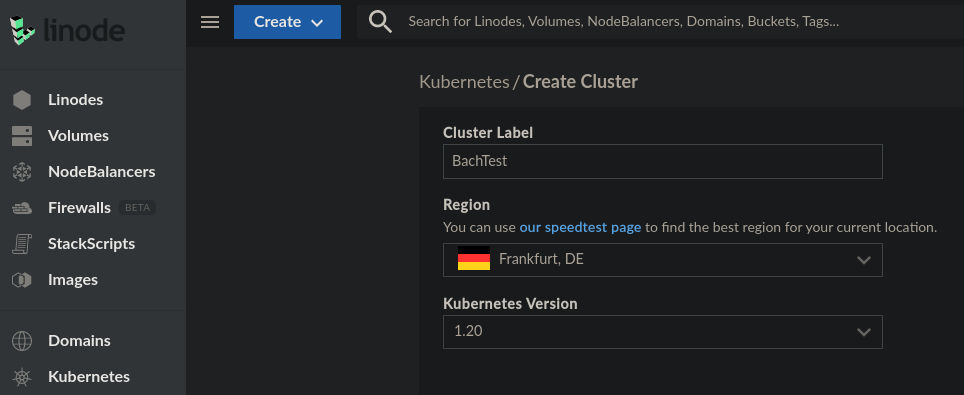
\includegraphics[width=\linewidth]{img/LinodeClusterNaam.png}
	\caption{Aanmaken Linode cluster}
	\label{fig:LinodeNaam}
\end{figure}

Vervolgens kunnen we nodes toevoegen aan de cluster. Voor dit onderzoek gaan we een kleinschalige cluster opzetten met 3 worker nodes en 1 master node. In figuur \ref{fig:LinodeAddNodes} zijn de verschillende soorten nodes die we kunnen toevoegen opgelijst. Tijdens deze scenario's zal gebruik gemaakt worden van 3 ``Linode 2GB'' nodes maar het is mogelijk om nodes van verschillende grotes in dezelfde cluster toe te voegen. De master node is niet meegerekend in deze 3 nodes maar word door Linode gratis aangeboden bij het opzetten van een K8s cluster.

\begin{figure}[ht]
	\centering
	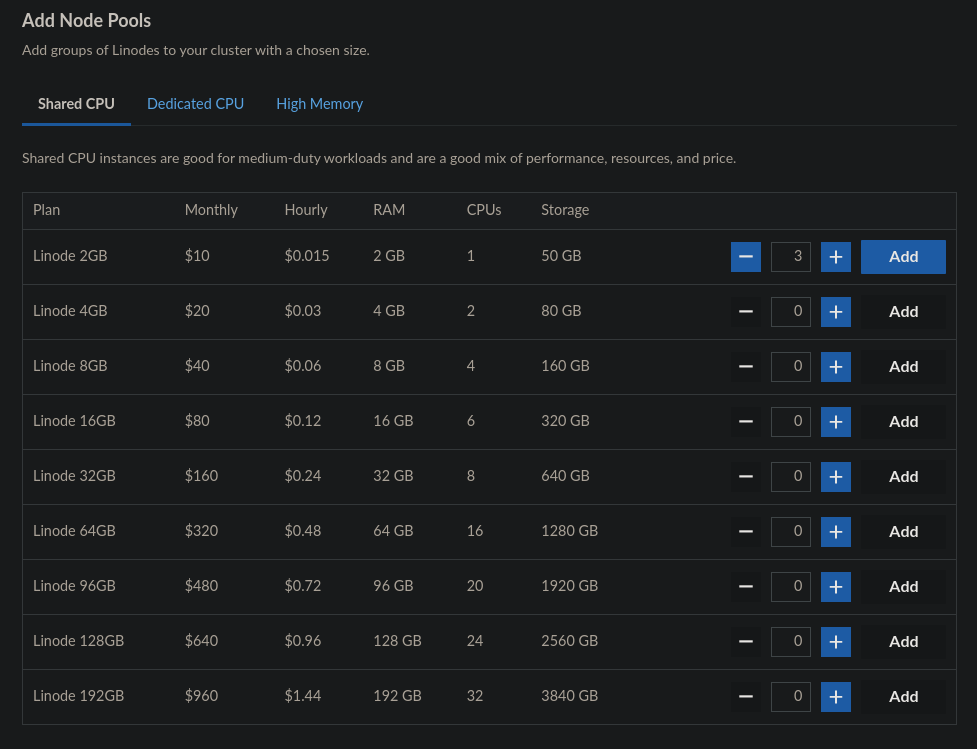
\includegraphics[width=\linewidth]{img/LinodeAddNodes.png}
	\caption{Toevoegen van nodes aan cluster}
	\label{fig:LinodeAddNodes}
\end{figure}

Als alle nodes zijn toegevoegd word de cluster aangemaakt. Linode zal dan in de achtergrond de gekozen nodes aanmaken alsook de master node klaarmaken voor gebruik. 

Eenmaal de cluster is aangemaakt en opgestart is moeten we deze nog configureren. Deze configuratie gebeurt via Kubectl in volgende stappen.

Als eerste moeten we het kubeconfig.yaml bestand downloaden van Linode. In dit bestand staan alle nodig details om te Kubectl te connecteren met onze cluster. De kubeconfig van onze net aangemaakte cluster ziet er uit zoals \ref{kubeconfig} (enkele waarden werden ingekort om de leesbaarheid te vergroten).

\begin{figure}[ht] \label{kubeconfig}
	\begin{minted}{yaml}
apiVersion: v1
kind: Config
preferences: {}

clusters:
- cluster:
    certificate-authority-data: LS0tLS1CRUdJTiBDRVJUSUZJQ0FURS0tLS0txvd0ZURVRNQkVHQTFVRQpBeE1LYTNWaVpYSnVaWFJsY3pDQ0FTSXdEUVlKS29aSWh2Y05BUUVCQlFBRGdnRVBBRENDQVFvQ2dn
    server: https://e08328fb-02d7-49a6-9f12-b4bdeb98510c.eu-central-2.linodelke.net:443
  name: lke25796

users:
- name: lke25796-admin
  user:
    as-user-extra: {}
    token: eyJhbGciOiJSUzI1NiIsImtpZCI6IlZ1a29MSDNqVVhXS1YyMjFNNVhJeHFjTFNXaXhwYVhNT3FWb2NjTWFOV2MifQ.eyJpc3MiOiJrdWJlcm5ldGVzL3NlcnZpY2VhY2NvdW50Iiwia3ViZ

contexts:
- context:
    cluster: lke25796
    namespace: default
    user: lke25796-admin
  name: lke25796-ctx

current-context: lke25796-ctx
	\end{minted}
		\caption{kubeconfig.yaml}
\end{figure}

Vervolgens moet het pad naar het bestand geëxporteerd worden naar de omgevingsvariabele ``KUBECONFIG'' met het volgende commando:
\begin{minted}{bash}
$ export KUBECONFIG=<pad naar file>/kubeconfig.yaml
\end{minted}

We kunnen testen of dit gelukt is door het volgende commando uit te voeren. Dit zou de 3 aangemaakte nodes in onze cluster moeten teruggeven.
\begin{minted}{bash}
$ kubectl get nodes
NAME                          STATUS   ROLES    AGE    VERSION
lke25332-32960-608682818f2e   Ready    <none>   6d4h   v1.20.5
lke25332-32960-60868281f030   Ready    <none>   6d4h   v1.20.5
lke25332-32960-608682824efd   Ready    <none>   6d4h   v1.20.5
\end{minted}


Nu Kubectl in contact staat met de ``kube-apiserver'' die op de master node staat, kunnen we beginnen met het configureren van onze cluster. Dit kan zowel met ``ad-hoc'' commando's als met zogenaamde deployements die werken via het ``principle of desired state''. In andere woorden, de deployements specificeren de verschillende aspecten van de cluster en K8s zorgt ervoor dat aan al deze specificaties wordt voldaan.

Een deployement is eigenlijk niets anders dan een YAML bestand waarin beschreven wordt hoe de cluster er moet gaan uitzien. Via het volgende commando wordt een deployement op een cluster gezet.
\begin{minted}{bash}
$ kubectl apply -f deployement.yaml
\end{minted}


	
\subsection{Gegevens- verzameling en verwerking}
\begin{itemize}
	\item Welke data er verzameld zal worden (CPU en RAM gebruik, Boot time, stability aka spikes per time) en waarom
 	\item Uitleg over hoe deze data zal verzameld worden(sysstat) en welke grafieken er zullen gebruikt worden om een vergelijking te kunnen maken (R code tonen).
\end{itemize}



\clearpage
\section{Scenario 1: Cluster opstelling zonder oog voor security}
\begin{itemize}
\item Basic Deployement van een statische website uitleggen aan de hand van commando's, screenshots en config files. 
\item Deployement YAML tonen en deels uitleggen
\item Service YAML tonen en deels uitleggen
\item Nodige gegevens uit de cluster halen met sysstat
\item Verzamelde gegevens verwerken met RStudio en grafieken/statistieken tonen en uitleggen.
\end{itemize}



\clearpage
\section{Scenario 2: Cluster opstelling met gebruik van best practices}
\begin{itemize}
	\item Basic Deployement van een statische website met best proctices uitleggen aan de hand van commando's, screenshots en config files. 
	\item Vooral RunAsUser en network policy's
	\item Deployement YAML tonen en best practices uitleggen
	\item Service YAML tonen en best practices uitleggen
	\item Nodige gegevens uit de cluster halen met sysstat
	\item Verzamelde gegevens verwerken met RStudio en grafieken/statistieken tonen en uitleggen
\end{itemize}


\clearpage
\section{Scenario 3: Cluster opstelling met security tools}
\begin{itemize}
	\item Basic Deployement van een statische website met enkele security tools uitleggen aan de hand van commando's, screenshots en config files. 
	\item Vooral Kubehunter en KubeBench uitleggen en praktisch voorstellen
	\item YAML files / commandos tonen en de werking uitleggen
	\item Deployement YAML tonen en best practices uitleggen
	\item Service YAML tonen en best practices uitleggen
	\item Nodige gegevens uit de cluster halen met sysstat
	\item Verzamelde gegevens verwerken met RStudio en grafieken/statistieken tonen en uitleggen
\end{itemize}
